\documentclass[12pt]{article}
\usepackage{graphicx}
\graphicspath{ {images/} }
\usepackage[spanish]{babel}
\usepackage[utf8]{inputenc}
\usepackage[backend=biber]{biblatex}
\bibliography{ref}
\usepackage[T1]{fontenc}
\usepackage{lmodern}

\begin{document}

\thispagestyle{empty}
\begin{center}
\begin{figure}[h]
\centering

\includegraphics[width=.6\textwidth]{logo.jpg}\\
\end{figure}

\vspace{1cm}
\Large \sc  Instituto Tecnológico y de Estudios Superiores de Monterrey
\\

\vspace{2.5cm}
\Large \bf
\emph{Actividad 1. Conceptos básicos de ciencia de datos}

\vspace{2.5cm}
\Large \bf Nombre del estudiante\\
\vspace{0.3cm}
\Large \bf Matrícula\\
\vspace{3.5cm}
\normalsize \sc \rightline{Ciencia y analítica de datos}
\vspace{0.3cm}
\normalsize \sc \rightline{Fecha}
\end{center}

\newpage

\section{Aprendizaje automático}
Lorem ipsum dolor sit amet, consectetur adipiscing elit, sed do eiusmod tempor incididunt ut labore et dolore magna aliqua. Tristique nulla aliquet enim tortor at auctor. Ipsum dolor sit amet consectetur adipiscing elit. Nunc mattis enim ut tellus. Imperdiet nulla malesuada pellentesque elit. Tortor condimentum lacinia quis vel eros donec ac. Sed faucibus turpis in eu mi bibendum neque. Sed nisi lacus sed viverra tellus in hac habitasse. Metus dictum at tempor commodo ullamcorper a. Ac ut consequat semper viverra nam libero justo laoreet \cite{1}. \\

Bibendum arcu vitae elementum curabitur vitae nunc. Ut placerat orci nulla pellentesque dignissim enim sit amet venenatis. Neque convallis a cras semper auctor neque vitae tempus quam. Facilisis sed odio morbi quis. Sit amet massa vitae tortor condimentum lacinia quis. Id eu nisl nunc mi ipsum faucibus vitae aliquet. Neque vitae tempus quam pellentesque nec nam. Ipsum consequat nisl vel pretium \cite{2}.\\

\section{Minería de datos}

Lorem ipsum dolor sit amet, consectetur adipiscing elit, sed do eiusmod tempor incididunt ut labore et dolore magna aliqua. Tristique nulla aliquet enim tortor at auctor. Ipsum dolor sit amet consectetur adipiscing elit. Nunc mattis enim ut tellus. Imperdiet nulla malesuada pellentesque elit. Tortor condimentum lacinia quis vel eros donec ac. Sed faucibus turpis in eu mi bibendum neque. Sed nisi lacus sed viverra tellus in hac habitasse. Metus dictum at tempor commodo ullamcorper a. Ac ut consequat semper viverra nam libero justo laoreet \cite{1}. \\

\section{Big data}
Lorem ipsum dolor sit amet consectetur adipiscing elit et sapien, himenaeos dictumst curabitur cras rhoncus dapibus lacinia orci malesuada, nisi ornare turpis purus hac placerat duis molestie. Potenti tincidunt curabitur urna litora a auctor, ornare euismod porttitor libero. Blandit eleifend bibendum ultricies molestie vel ad quis lacus orci libero, a ridiculus eu feugiat litora malesuada diam faucibus magnis, ullamcorper aenean tempus imperdiet sagittis primis eros nulla ante \cite{1}.


\section{Analítica de datos}

Phasellus ullamcorper condimentum neque sodales fusce sapien quisque suscipit tellus, cum lacinia diam elementum facilisi orci egestas non nisi lobortis, pharetra varius duis maecenas hendrerit accumsan inceptos penatibus. Venenatis ante taciti rutrum tempus montes imperdiet purus velit platea laoreet suscipit, dapibus nisl auctor aenean egestas id molestie quisque pretium mauris. Dictumst nullam class vel commodo neque nunc ligula non, placerat mauris vivamus nulla pretium in dapibus, porta hac nisi condimentum natoque duis donec \cite{2}. 


\section{¿Cómo se relaciona cada uno de estos 4 elementos con la ciencia de datos?}

Sollicitudin quisque per lacus habitasse imperdiet fames duis fringilla rhoncus facilisis, ac scelerisque nullam massa et vel lobortis netus nibh congue magnis, viverra litora sociis curae luctus dictumst suspendisse quis cum. Iaculis sagittis nisl mollis viverra malesuada netus conubia tellus velit cubilia porta taciti, sem penatibus enim maecenas ac neque curabitur luctus dis tempus sociosqu nisi non, suspendisse accumsan sapien vestibulum turpis quisque facilisis quam dui tortor bibendum. \\

Litora sociis sem parturient mi faucibus non fusce, primis diam malesuada sodales egestas nullam fermentum, lacus tellus dui ad himenaeos nam. Ultrices gravida cursus hac pellentesque pretium parturient leo, a quam phasellus aliquam id nunc proin tellus, vestibulum habitasse arcu ad torquent purus inceptos, dignissim etiam quisque duis massa pulvinar. Himenaeos semper eget ultrices venenatis mattis luctus rutrum hac cursus fermentum tellus euismod dictumst viverra non, habitasse vestibulum cras porta inceptos nulla fringilla mauris integer facilisis facilisi bibendum egestas. 

% Ejemplo de cómo incluir una figura (no cuentan en la extensión de las dos cuartillas)
\begin{figure}[h]
\centering{
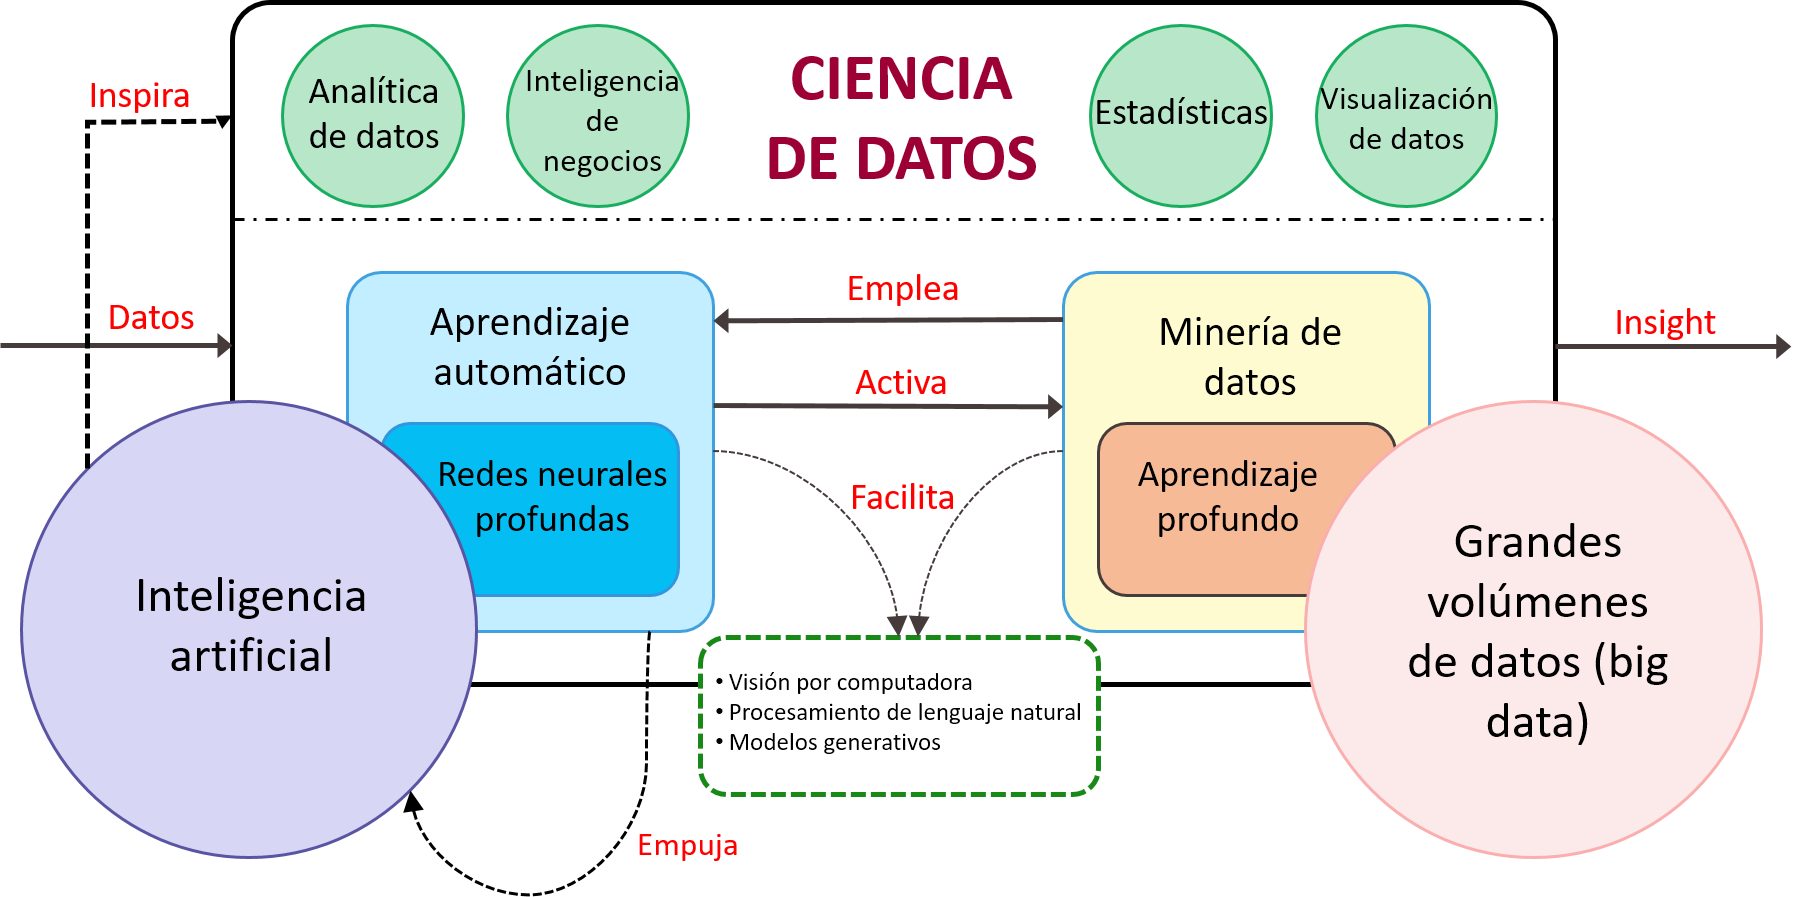
\includegraphics[width=1\textwidth]{imagen.png}\\
\caption{Diagrama de ciencia de datos \cite{3}}}
\end{figure}

\newpage
\begin{thebibliography}{a}

% Ejemplo de libro
\bibitem{goossens93} 
Michel Goossens, Frank Mittelbach and Alexander Samarin, \emph{The LaTeX Companion}, Addison-Wesley, 1993.

% Ejemplo de artículo
\bibitem{einstein}
Albert Einstein. \emph{Zur Elektrodynamik bewegter K{\"o}rper}.
\emph{Annalen der Physik}, 322(10):891--921, 1905.

% Ejemplo de página web
\bibitem{website_example} 
The Data Science Puzzle, Explained. KDnuggets. \\ \url{https://www.kdnuggets.com/2016/03/data-science-puzzle-explained.html} (visitado 15-04-2024)

\end{thebibliography}

\end{document}
